% Written by make_results.py from wave3_heldout_20261025T1625Z/<suite>/report/metrics.json. Do not edit.
% Share of recorded runs that met the case's outcome, per policy and suite.
\documentclass[border=3pt]{standalone}
% Shared style of every Plan B figure (the deck, the poster and the documentation).
% Type is near-black and grey on white. UMB blue is the brand and the system. One warm accent
% marks tension only (the incoming message, the clock). Green marks only an accepted receipt or
% a met run. Square corners, thin rules, no shadows, no gradients.
\usepackage[T1]{fontenc}
\usepackage[scaled]{helvet}
\renewcommand{\familydefault}{\sfdefault}
\usepackage{tikz}
\usepackage{pgfplots}
\pgfplotsset{compat=1.18}
\usepackage{fontawesome5}
\hyphenpenalty=10000
\exhyphenpenalty=10000
\usetikzlibrary{arrows.meta,positioning,calc,fit,backgrounds}

% Colours
\definecolor{primary}{HTML}{08457E}   % UMB blue: the system, Plan B's own policy
\definecolor{primarysoft}{HTML}{E7EEF5}
\definecolor{accent}{HTML}{FF791F}    % tension only: the message, the gap, the one missed run
\definecolor{accentsoft}{HTML}{FFEBDC}
\definecolor{umbblue}{HTML}{005A8B}   % UMB blue: the three idea marks and structure
\definecolor{navy}{HTML}{132245}      % title bands, the receipt, the dark close
\definecolor{ground}{HTML}{EEF2F6}    % the light blue-grey ground behind white cards
\definecolor{ok}{HTML}{2E7D32}        % an accepted receipt, a met run
\definecolor{oksoft}{HTML}{E5F1E6}
\definecolor{ink}{HTML}{1F1F1F}
\definecolor{muted}{HTML}{6B6B6B}
\definecolor{quiet}{HTML}{9A9A9A}     % other policies, context
\definecolor{rulegrey}{HTML}{C4C4C4}
\definecolor{gridgrey}{HTML}{E4E4E4}
\definecolor{faint}{HTML}{F4F4F4}

\tikzset{
  >={Stealth[length=2.4mm,width=1.8mm]},
  every picture/.style={line cap=butt, line join=miter},
  % text styles
  hd/.style={font=\bfseries, text=ink, align=left},
  sub/.style={text=muted, align=left},
  % shapes: square or 1 pt corners, thin rules
  card/.style={draw=rulegrey, line width=0.5pt, fill=white, rounded corners=1pt, inner sep=5pt, align=left, text=ink},
  sys/.style={draw=primary, line width=0.8pt, fill=white, rounded corners=1pt, inner sep=5pt, align=center, text=ink},
  sysfill/.style={draw=primary, line width=0.8pt, fill=primary, rounded corners=1pt, inner sep=5pt, align=center, text=white},
  warm/.style={draw=accent, line width=0.8pt, fill=accentsoft, rounded corners=1pt, inner sep=5pt, align=left, text=ink},
  receipt/.style={draw=ok, line width=0.8pt, fill=oksoft, rounded corners=1pt, inner sep=5pt, align=left, text=ink},
  planned/.style={draw=muted, line width=0.6pt, dash pattern=on 3pt off 2pt, fill=white, rounded corners=1pt, inner sep=5pt, align=left, text=muted},
  % connectors
  link/.style={->, draw=muted, line width=0.6pt},
  syslink/.style={->, draw=primary, line width=0.9pt},
  oklink/.style={->, draw=ok, line width=0.9pt},
  warmlink/.style={->, draw=accent, line width=0.9pt},
  nextlink/.style={->, draw=muted, line width=0.6pt, dash pattern=on 3pt off 2pt},
}

% Charts: a real axis, few light gridlines, no frame on the top and right.
\pgfplotsset{
  planb/.style={
    axis line style={draw=muted, line width=0.5pt},
    tick style={draw=muted, line width=0.5pt},
    major tick length=3pt,
    tick label style={text=ink, /pgf/number format/assume math mode=true},
    label style={text=ink},
    title style={font=\bfseries, text=ink},
    grid style={draw=gridgrey, line width=0.4pt},
    every axis plot/.append style={line width=0.6pt},
    legend style={draw=none, fill=none, text=ink},
    legend cell align=left,
  },
}

% The three idea marks, the same in the deck, the poster and the report.
% 1 Check the fact (a magnifier), 2 Pick only what fits (a funnel that keeps what fits),
% 3 Leave a receipt (a receipt slip). Always in UMB blue unless the panel is navy.
\providecommand{\markcheck}{\faSearch}
\providecommand{\markfits}{\faFilter}
\providecommand{\markreceipt}{\faReceipt}
% The three points of "Why Plan B": safer shows the three marks together, more flexible a laptop,
% more personal a set of sliders.
\providecommand{\marksafer}{\faSearch\,\faFilter\,\faReceipt}
\providecommand{\markflexible}{\faLaptop}
\providecommand{\markpersonal}{\faSlidersH}

\begin{document}
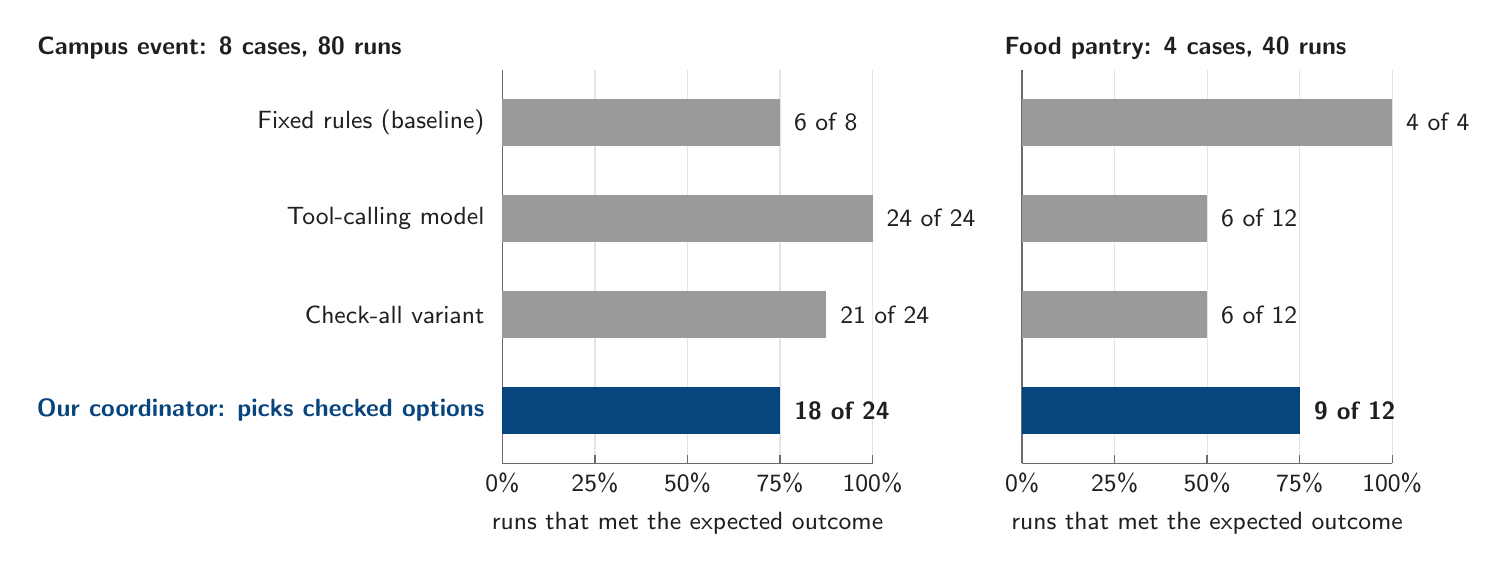
\begin{tikzpicture}[font=\small]
\begin{axis}[planb,
  name=campus,
  scale only axis,
  width=4.7cm,
  height=5.0cm,
  xbar, bar width=17pt,
  xmin=0, xmax=100, xtick={0,25,50,75,100},
  xticklabels={0\%,25\%,50\%,75\%,100\%},
  xmajorgrids, axis x line*=bottom, axis y line*=left,
  ytick={1,2,3,4}, y dir=reverse, ymin=0.45, ymax=4.55, ytick style={draw=none},
  yticklabels={{Fixed rules (baseline)},{Tool-calling model},{Check-all variant},{\bfseries\color{primary}Our coordinator: picks checked options}},
  xlabel={runs that met the expected outcome},
  clip=false]
\addplot[draw=none, fill=quiet, bar shift=0pt] coordinates {(75.0000,1)};
\node[anchor=west, text=ink] at (axis cs:75.0000,1) {\,6 of 8};
\addplot[draw=none, fill=quiet, bar shift=0pt] coordinates {(100.0000,2)};
\node[anchor=west, text=ink] at (axis cs:100.0000,2) {\,24 of 24};
\addplot[draw=none, fill=quiet, bar shift=0pt] coordinates {(87.5000,3)};
\node[anchor=west, text=ink] at (axis cs:87.5000,3) {\,21 of 24};
\addplot[draw=none, fill=primary, bar shift=0pt] coordinates {(75.0000,4)};
\node[anchor=west, text=ink] at (axis cs:75.0000,4) {\bfseries\,18 of 24};
\end{axis}
\node[anchor=south west, text=ink] at (campus.outer north west) {\bfseries Campus event: 8 cases, 80 runs};
\begin{axis}[planb,
  name=pantry, at={(campus.south east)}, anchor=south west, xshift=1.9cm,
  scale only axis,
  width=4.7cm,
  height=5.0cm,
  xbar, bar width=17pt,
  xmin=0, xmax=100, xtick={0,25,50,75,100},
  xticklabels={0\%,25\%,50\%,75\%,100\%},
  xmajorgrids, axis x line*=bottom, axis y line*=left,
  ytick={1,2,3,4}, y dir=reverse, ymin=0.45, ymax=4.55, ytick style={draw=none},
  yticklabels={},
  xlabel={runs that met the expected outcome},
  clip=false]
\addplot[draw=none, fill=quiet, bar shift=0pt] coordinates {(100.0000,1)};
\node[anchor=west, text=ink] at (axis cs:100.0000,1) {\,4 of 4};
\addplot[draw=none, fill=quiet, bar shift=0pt] coordinates {(50.0000,2)};
\node[anchor=west, text=ink] at (axis cs:50.0000,2) {\,6 of 12};
\addplot[draw=none, fill=quiet, bar shift=0pt] coordinates {(50.0000,3)};
\node[anchor=west, text=ink] at (axis cs:50.0000,3) {\,6 of 12};
\addplot[draw=none, fill=primary, bar shift=0pt] coordinates {(75.0000,4)};
\node[anchor=west, text=ink] at (axis cs:75.0000,4) {\bfseries\,9 of 12};
\end{axis}
\node[anchor=south west, text=ink] at (pantry.outer north west) {\bfseries Food pantry: 4 cases, 40 runs};
\end{tikzpicture}
\end{document}
